
% tipo de documento
\documentclass{article}

% formato de página
\usepackage[margin=1.5cm, letterpaper]{geometry}

% idioma de los macros
\usepackage[spanish]{babel}
\usepackage[utf8]{inputenc}

% vínculos
\usepackage{hyperref}

% manejo de ecuaciones
\usepackage{amsmath}

% manejo de figuras
\usepackage{graphicx}
\usepackage{float}

% texto del documento
\begin{document}
    \title{
        Organización y Arquitectura de Computadoras \\
        Práctica 7: Convención de llamadas a subrutinas \\
    }
    \date{
        14 de abril del 2019
    }
    \author{
        Sandra del Mar Soto Corderi \\
        Edgar Quiroz Castañeda
    }
    \maketitle

    \section{Preguntas}
    \begin{enumerate}
    
    %1
    \item {
    ¿Qué utilidad tiene el registro $\textbf{\$fp}$? ¿Se puede prescindir de el?\\
	
	El registro $\textbf{\$fp}$ es el que corresponde al Apuntador del marco, el cual guarda la dirección de la última palabra del marco. Un apuntador de marco, si es utilizado, apunta a una dirección en la pila donde los argumentos y variables locales para una función(subrutina) invocada son localizadas. Este apuntador es establecido en la entrada de una función y se mantiene constante en la ejecución de la función invocada.\\
	
	Sí se puede prescindir del fp. No todos los procesadores tienen los recursos de hardware para implementar un apuntador de marco y algunas implementaciones donde se sabe exactamente la distancia del marco, no quieren tener la sobrecarga adicional de mantenerlo.\\  
	}
	%2
	\item {
	Definimos como \textbf{subrutina nodo} a una subrutina que realiza una o más
	invocaciones a otras subrutinas y como \textbf{subrutina hoja} a una subrutina
	que no realiza llamadas a otras subrutinas.
	
		\begin{enumerate}
			%a
			\item {
			¿Cuál es el tamaño mínimo que puede tener un marco para una subrutina nodo? ¿Bajo qué condiciones ocurre?\\
			
			El tamaño mínimo que puede tener un marco para una subrutina nodo es dos veces el tamaño del marco original, asumiendo que es llamada una vez, que sería de 32 bytes.\\
			}
			%b
			\item {
			¿Cuál es el tamaño mínimo que puede tener un marco para una subrutina hoja? ¿Bajo qué condiciones ocurre?\\
			
			El tamaño mínimo que puede tener un marco para una subrutina nodo es el tamaño del marco original, que sería de 32 bytes.\\
			
			}
		\end{enumerate}
		
	
	}
	
		
	%3
	\item{
	Considera el siguiente pseudocódigo de la figura 3. En donde a[5] es un
	arreglo de tamaño 5 y “...” son otras acciones que realiza la rutina, además, supón que en la función B se realizan cambios en los registros $\$s0, \$s1$
	y $\$s2$. Bosqueja la pila de marcos después del preámbulo de la función B.\\
	
	\begin{figure}[H]
		\centering
		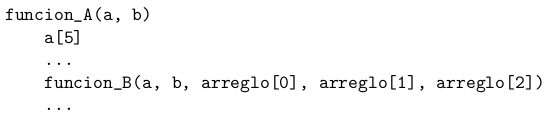
\includegraphics[scale=0.5]{Figura1.png}
		\caption{Rutina con llamado a subrutina}
	\end{figure}


	La pila de marcos sería:\\
	
	\begin{figure}[H]
		\centering
		\includegraphics[scale=0.5]{Figura2.png}
		\caption{Pila de marcos de la función B}
	\end{figure}
	
	}
        
    \end{enumerate}


    \begin{thebibliography}{1}
       
    \end{thebibliography}
\end{document}